\documentclass[11pt,a4paper]{article}

\usepackage{url,,}
\usepackage{graphicx}
\usepackage{hyperref}
\usepackage{amsfonts}
\usepackage{amssymb}
\usepackage{amsmath}
\usepackage{amsfonts}
\usepackage{amssymb}
\usepackage{amsmath}
\usepackage{multirow}
\usepackage{listings}
\usepackage{fullpage}
\usepackage{fancyhdr,a4wide}
\usepackage{makeidx}
\usepackage{placeins}
\usepackage[procnames,noindent]{lgrind}

\lstset{ %
language=C,                % choose the language of the code
basicstyle=\footnotesize,       % the size of the fonts that are used for the code
showstringspaces=false,         % underline spaces within strings
numbers=left,                   % where to put the line-numbers
%numberstyle=\footnotesize,      % the size of the fonts that are used for the line-numbers
%stepnumber=1,                   % the step between two line-numbers. If it's 1 each line will be numbered
%numbersep=5pt,                  % how far the line-numbers are from the code
%backgroundcolor=\color{white},  % choose the background color. You must add \usepackage{color}
showspaces=false,               % show spaces within strings adding particular underscores
showtabs=false,                 % show tabs within strings adding particular underscores
escapeinside={\%*}{*)}          % if you want to add a comment within your code
}

\begin{document}	

%\begin{titlepage}
%
%\thispagestyle{fancy}
%\lhead{}
%\chead{
%\large{\textit{
%Department of Mathematics\\
%Technical University of Denmark}}}
%\rhead{}
%\rule{0pt}{50pt}
%\vspace{3cm}
%
%\begin{center}
% 	\huge{\textbf{The HiTag2 Stream Cipher}}\\
% 	\vspace{1cm}
%\end{center}
%
%\vspace{4cm}
%
%\begin{center}
%	\LARGE{Rajesh Bachani \\(s061332)}\\
%\end{center}
%\cfoot{\today}
%\end{titlepage}
\newcommand{\TITLE}{The HiTag2 Stream Cipher}
%
\oddsidemargin 0.0in \evensidemargin 1.0in \textwidth 6.0in
%
\begin{titlepage}
\title{\TITLE}
%
\author{Rajesh Bachani \thanks{Email:{\texttt{s061332@student.dtu.dk}}}\\
%
\small Department of Mathematics, Technical University of Denmark\\
\small \today}
\date{}
\end{titlepage}

\maketitle

%-----------------------------------------------------------
\section{Cipher Description}
The components of the HiTag2 stream cipher are outlined below. 
\begin{itemize}
\item 48 bit Key
\item 32 bit Serial ID
\item 32 bit Initialization Vector (IV)
\item 48 bit internal state with linear update function (basically, a Linear Feedback Shift Register or LFSR)
\item Non-linear output function based on multiplexor, with fixed data bits and address bits depending on the current internal state
\end{itemize}

The entire setup of the keystream generator is done in two phases. The first phase is the initialization of the LFSR, while the second is the setup of the LFSR. Once the LFSR is set, the keystream is ready to be generated from the internal state.\\ Important note: unless mentioned otherwise, all the bit numbers mentioned in the following description are based on index values starting from 0, and not 1. 

\subsection{LFSR Initialization}

The initialization step of the LFSR is straightforward. Instead of initializing the LFSR with zeros, the bits are initialized with the Serial ID and initial part of the secret key. The 32 bits of the Serial ID (from lsb to msb) are stored in the first 32 bits of the LFSR. Then, the first 16 bits of the secret key are stored in the remaining 16 bits of the LFSR. With this the initialization of the LFSR is complete, as also shown in figure \ref{fig:hitag2-1}. 

\begin{figure}[h]
	\centering
		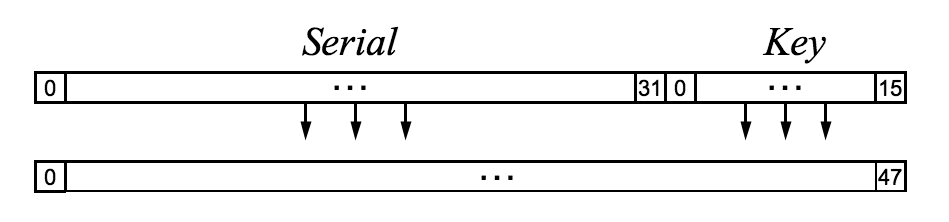
\includegraphics[width=6in]{./hitag2-1.PNG}
	\caption{LFSR Initialization}	
	\label{fig:hitag2-1}
\end{figure}

\subsection{LFSR Setup}

During the setup of the LFSR, the remaining bits of the secret key and the IV bits are used. The bits in the LFSR are shifted to the left in every clock cycle, and a new value is stored in the rightmost bit. In every clock cycle, an xor of three bits (one bit from the remaining part of the key (from bit 16 to 47), one bit from the IV (from bit 0 to 31) and the output bit from the non-linear output function) is written at the rightmost bit of the LFSR. After 32 clock cycles, the internal state is prepared for keystream generation. This is shown in figure \ref{fig:hitag2-2}.

\FloatBarrier
\begin{figure}[h]
	\centering
		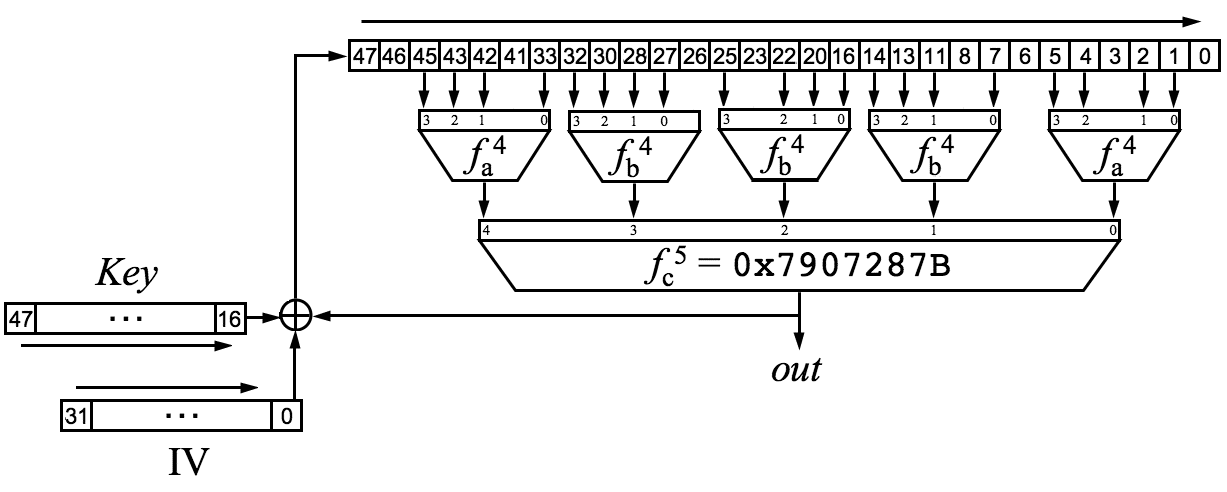
\includegraphics[width=6in]{./hitag2-2.PNG}
	\caption{LFSR Setup Phase}	
	\label{fig:hitag2-2}
\end{figure}
\FloatBarrier

The output function is basically a multiplexor with fixed data bits. Three multiplexor functions are used in the output function, and these are called $f_a^4$, $f_b^4$ and $f_c^5$. The different instances of these functions used are described below.

\paragraph{Function $f_a^4$}
\begin{itemize}
\item Data Bits: 0x2C79
\item Address Bits: LFSR bits (1, 2, 4, 5)
\end{itemize}

\paragraph{Function $f_b^4$}
\begin{itemize}
\item Data Bits: 0x6671
\item Address Bits: LFSR bits (7, 11, 13, 14)
\end{itemize}

\paragraph{Function $f_b^4$}
\begin{itemize}
\item Data Bits: 0x6671
\item Address Bits: LFSR bits (16, 20, 22, 25)
\end{itemize}

\paragraph{Function $f_b^4$}
\begin{itemize}
\item Data Bits: 0x6671
\item Address Bits: LFSR bits (27, 28, 30, 32)
\end{itemize}

\paragraph{Function $f_a^4$}
\begin{itemize}
\item Data Bits: 0x2C79
\item Address Bits: LFSR bits (33, 42, 43, 45)
\end{itemize}

\paragraph{Function $f_c^5$}
\begin{itemize}
\item Data Bits: 0x7907287B
\item Address Bits: Output bits from 5 multiplexor functions $f_a^4$, $f_b^4$, $f_b^4$, $f_b^4$, $f_a^4$ described above. 
\end{itemize}

Hence, in the setup phase, this output bit from the function $f_c^5$ is xor'ed with the key and IV bits for 32 cycles and written to the rightmost bit of the LFSR, as mentioned previously. 


\subsection{Keystream Generation}
The output from the function $f_c^5$ constitutes the keystream. During the keystream generation, the internal state is updated linearly, in the following fashion: an xor of the taps of the LFSR (which are bits 0, 2, 3, 6, 7, 8, 16, 22, 23, 26, 30, 41, 42, 43, 46 and 47) is written to the rightmost bit of the LFSR in every clock cycle. This is shown in figure \ref{fig:hitag2-3}.

\FloatBarrier
\begin{figure}[h]
	\centering
		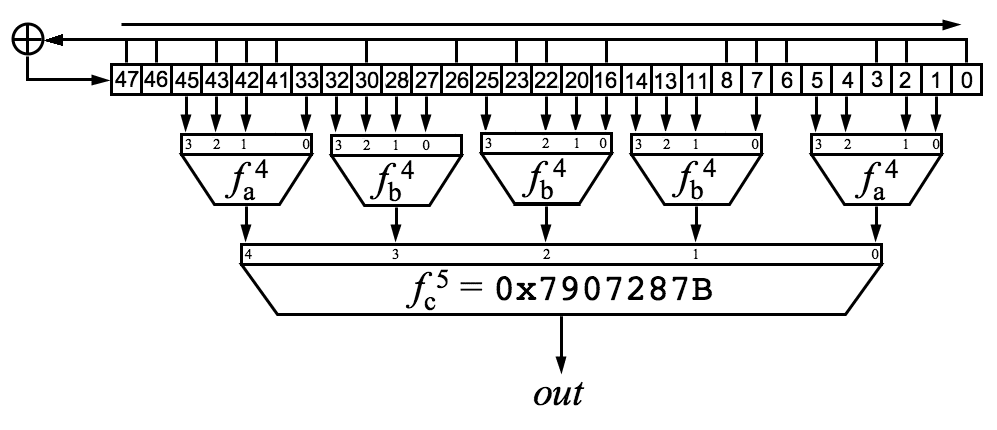
\includegraphics[width=6in]{./hitag2-3.PNG}
	\caption{Keystream Generation}	
	\label{fig:hitag2-3}
\end{figure}
\FloatBarrier

\section{HiTag2 C Program}
\lstinputlisting[columns=fullflexible] {./hitag2.c}

\newpage
\nocite{datasheet}
\nocite{code}
\bibliography{HiTag2}
\bibliographystyle{plain}

\end{document}